% anhang.tex
\chapter{Anhang}
\section{Plots der BLAST-Analyse der Individuen B und C}
%\begin{figure}[]
%	\begin{minipage}[b]{.49\linewidth}
%	\subfigure{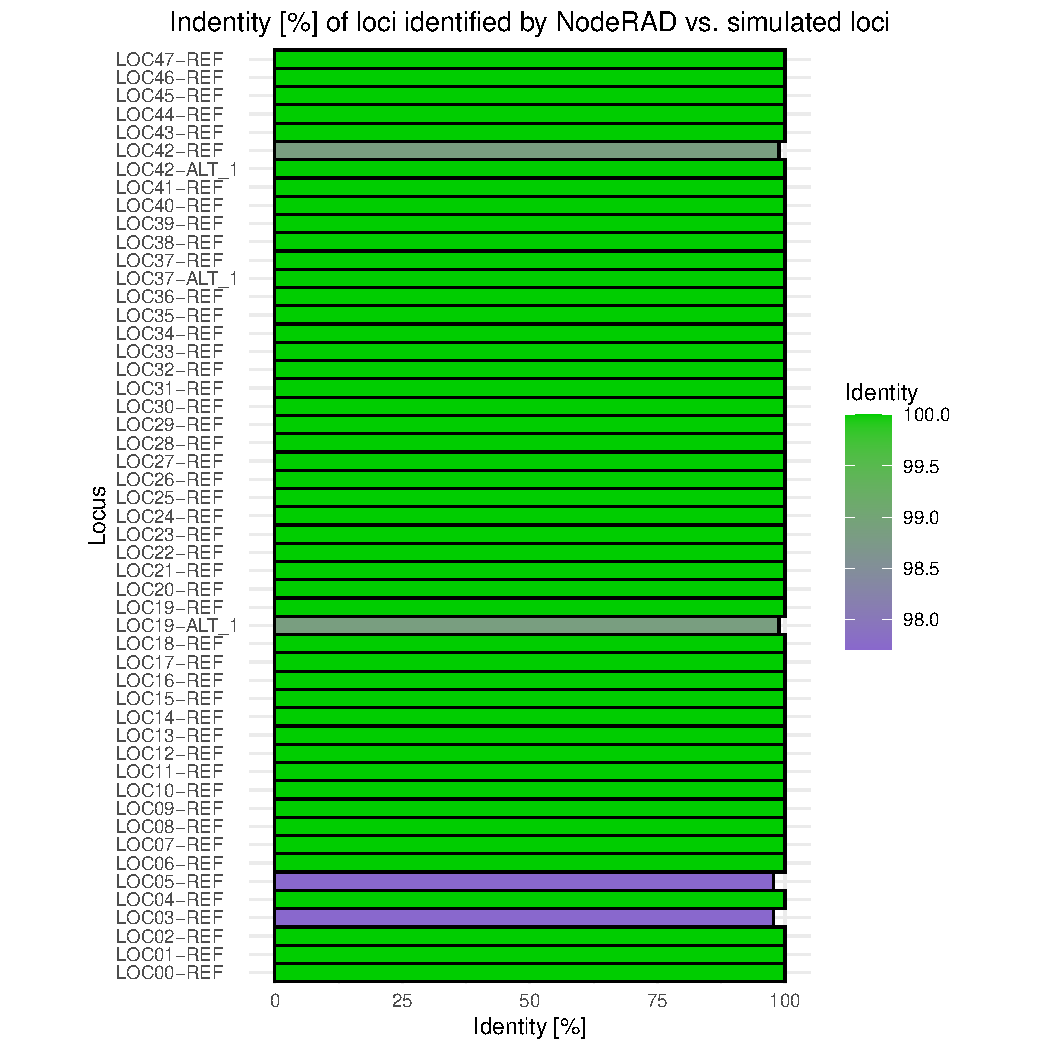
\includegraphics[width=\linewidth]{bilder/evaluation/perc_ident/B.plot_loci.pdf}}
%	\centering{Individuum B.}
%	\end{minipage}
%	\begin{minipage}[b]{.49\linewidth}
%	\subfigure{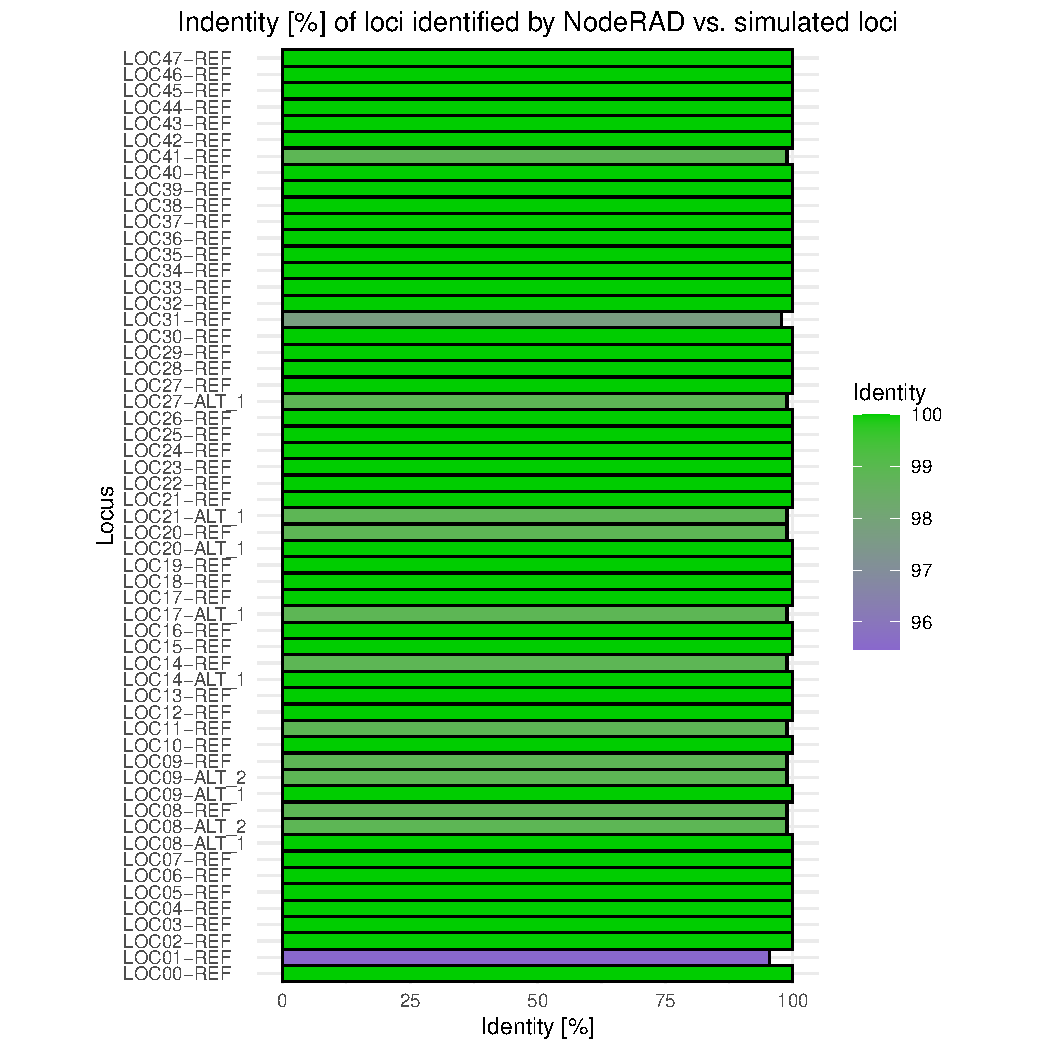
\includegraphics[width=\linewidth]{bilder/evaluation/perc_ident/C.plot_loci.pdf}}
%	\centering{Individuum C.}
%	\end{minipage}
%	\caption{{Sequenzähnlichkeit der durch NodeRAD bestimmten Loci gegenüber den simulierten Loci}}
%	\label{fig:ident_B_C}
%\end{figure}

\begin{figure}[H]
	\begin{center}
		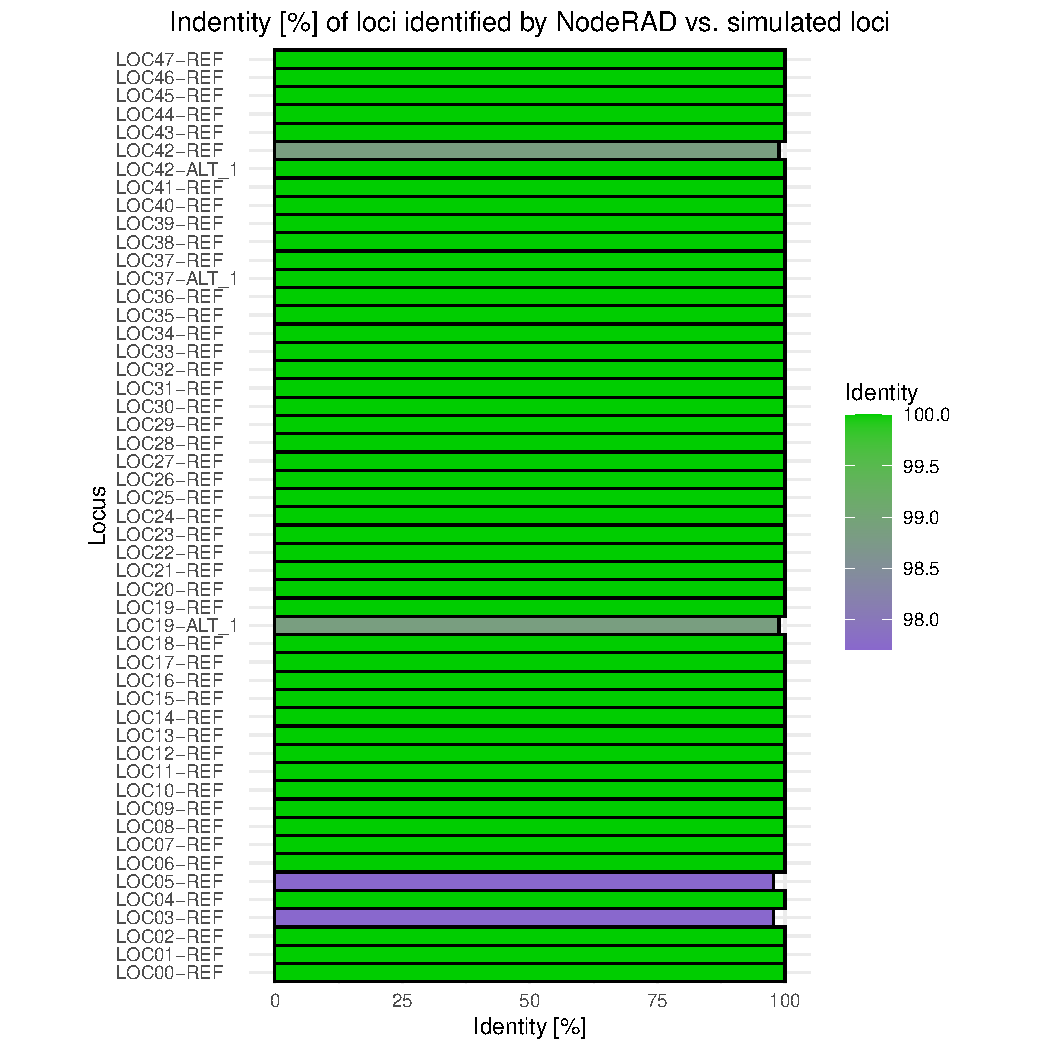
\includegraphics[height=16cm]{bilder/evaluation/perc_ident/B.plot_loci.pdf}
		\caption{Individuum B: Sequenzähnlichkeit (Identität in $ \% $) der durch NodeRAD bestimmten Loci gegenüber den simulierten Loci.}
	\end{center}
\end{figure}

\begin{figure}[H]
	\begin{center}
		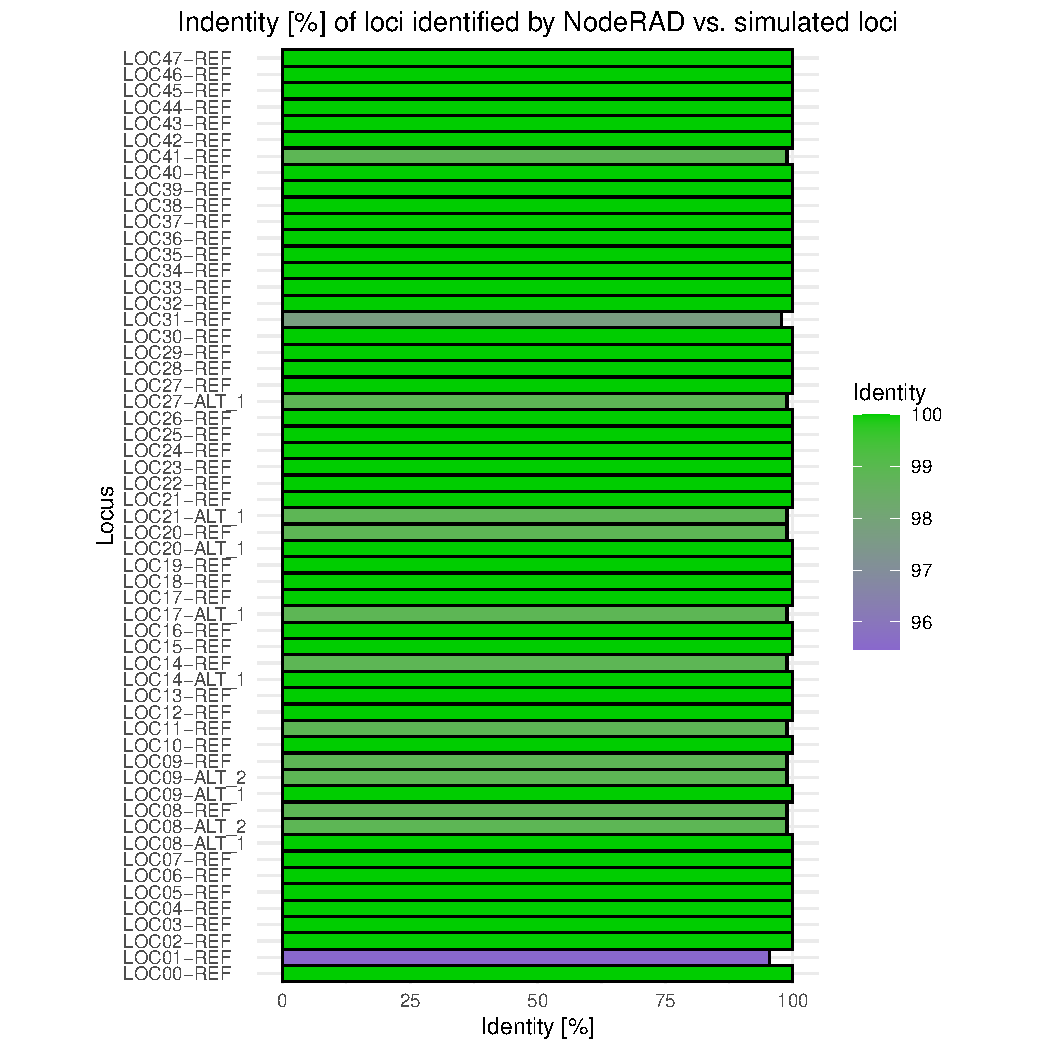
\includegraphics[height=16cm]{bilder/evaluation/perc_ident/C.plot_loci.pdf}
		\caption{Individuum C: Sequenzähnlichkeit (Identität in $ \% $) der durch NodeRAD bestimmten Loci gegenüber den simulierten Loci.}
	\end{center}
\end{figure}

\begin{figure}[H]
	\begin{center}
		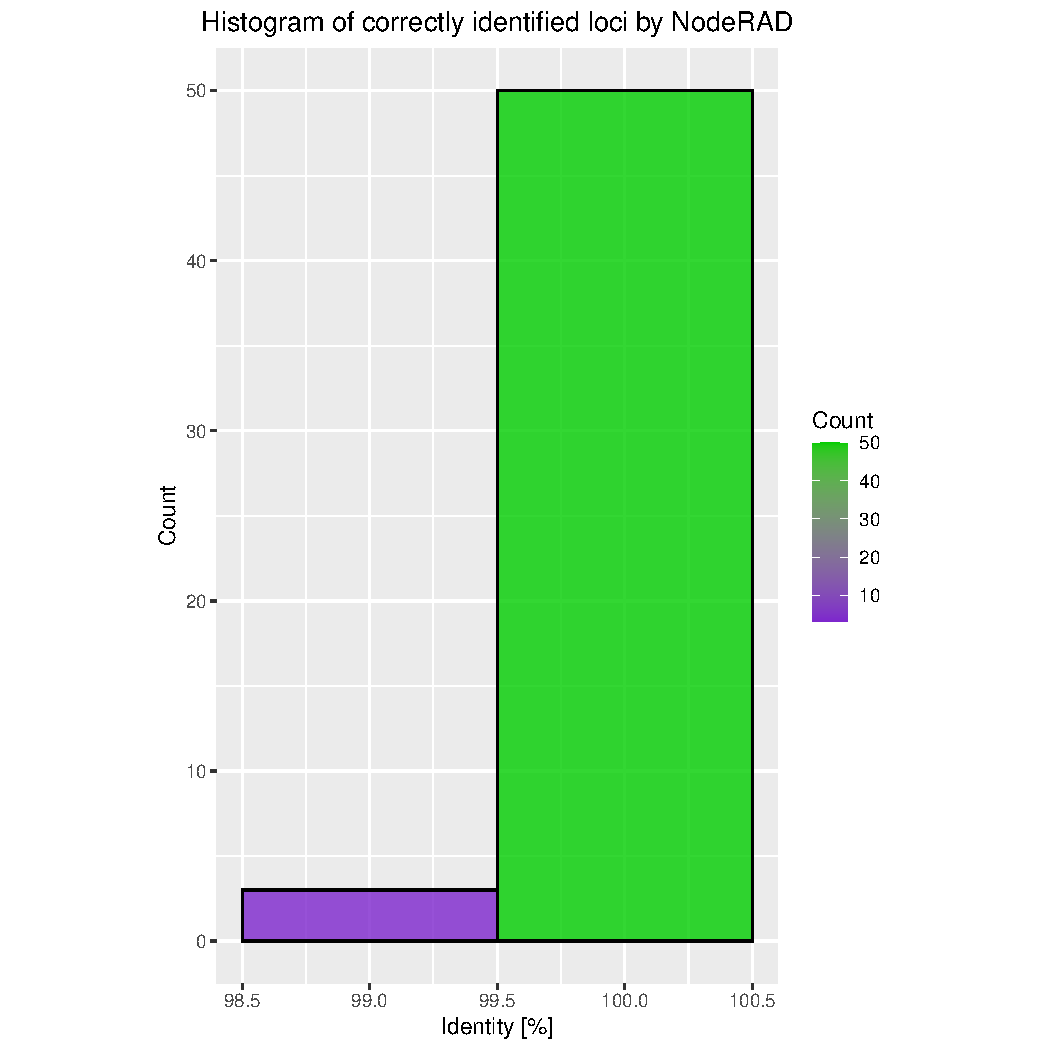
\includegraphics[height=16cm]{bilder/evaluation/hist_perc_ident/B.plot_hist.pdf}
		\caption{Individuum B: Anzahl der durch NodeRAD bestimmten Loci hinsichtlich der Sequenzählichkeit (Identität in $ \% $) zu den simulierten Loci}
	\end{center}
\end{figure}

\begin{figure}[H]
	\begin{center}
		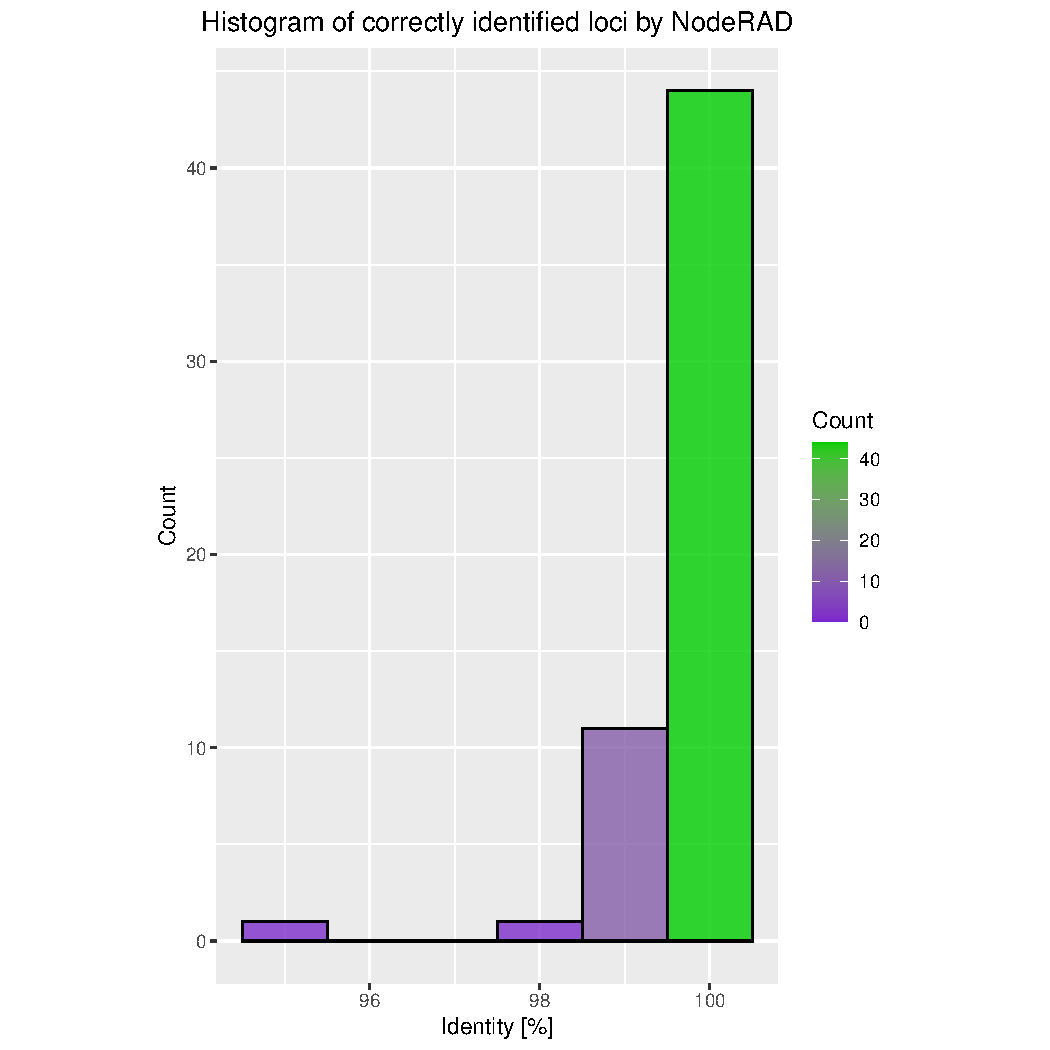
\includegraphics[height=16cm]{bilder/evaluation/hist_perc_ident/C.plot_hist.pdf}
		\caption{Individuum C: Anzahl der durch NodeRAD bestimmten Loci hinsichtlich der Sequenzählichkeit (Identität in $ \% $) zu den simulierten Loci}
	\end{center}
\end{figure}

\begin{figure}[H]
	\begin{center}
		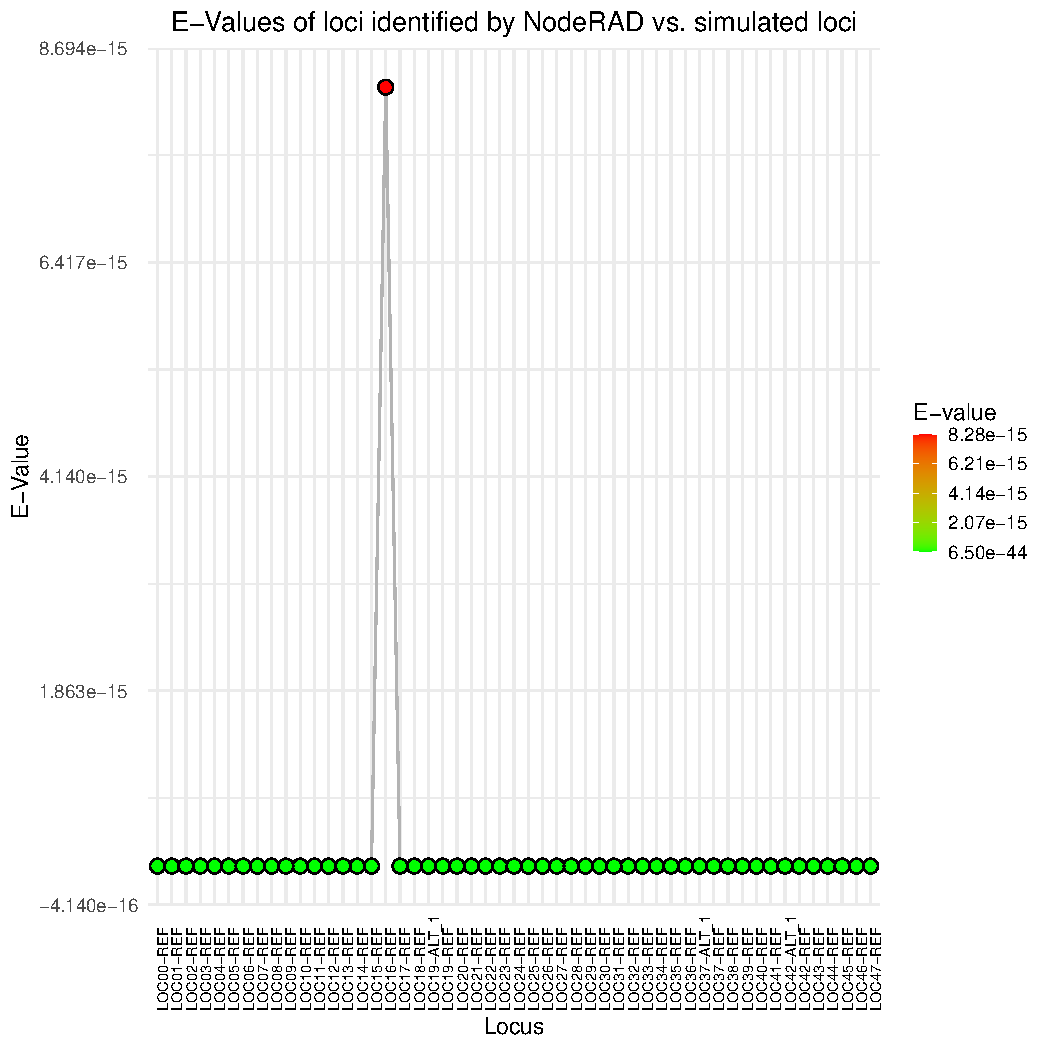
\includegraphics[height=16cm]{bilder/evaluation/evalues/B.plot_evalues.pdf}
		\caption{Individuum B: E-Values aus dem Vergleich der durch NodeRAD bestimmten Loci mit den simulierten Loci}
	\end{center}
\end{figure}

\begin{figure}[H]
	\begin{center}
		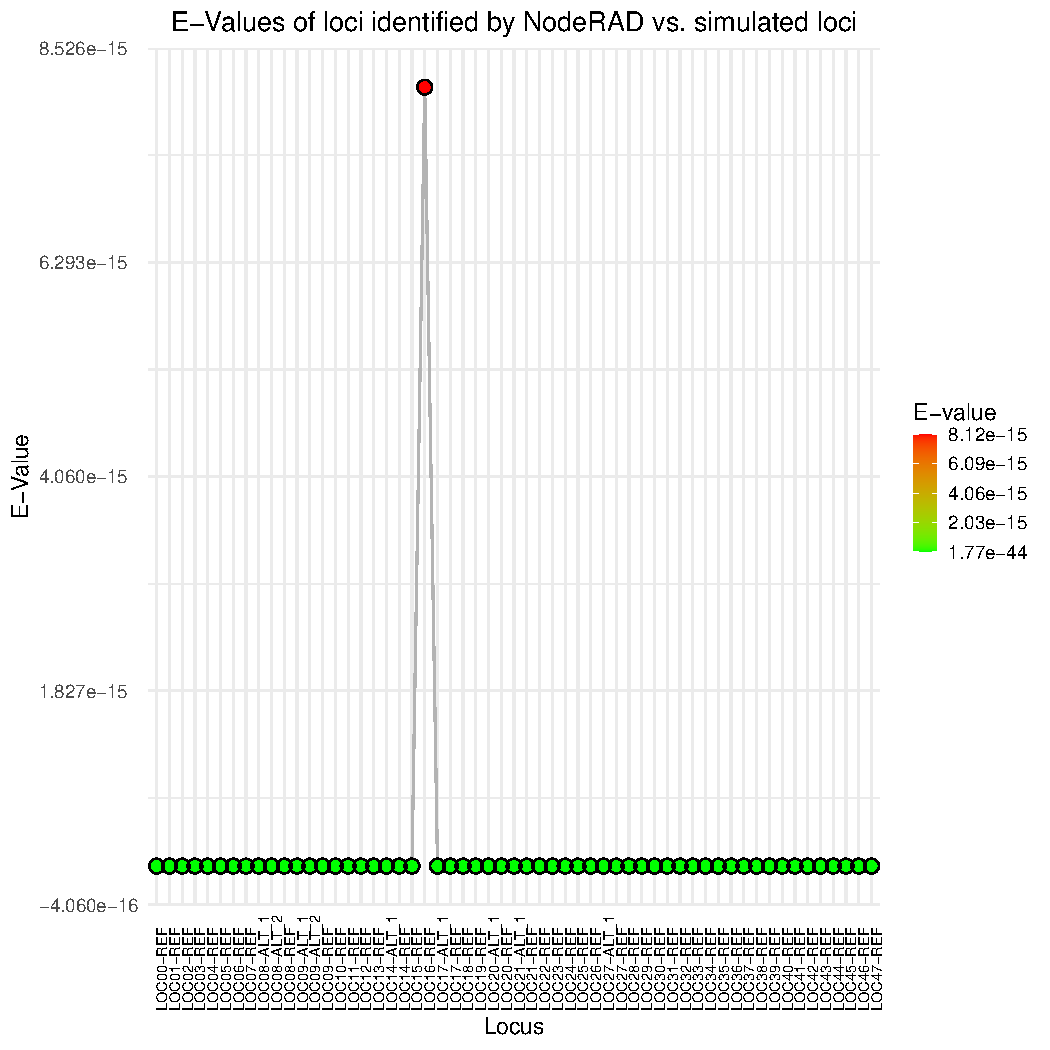
\includegraphics[height=16cm]{bilder/evaluation/evalues/C.plot_evalues.pdf}
		\caption{Individuum C: E-Values aus dem Vergleich der durch NodeRAD bestimmten Loci mit den simulierten Loci}
	\end{center}
\end{figure}

\begin{figure}[H]
	\begin{center}
		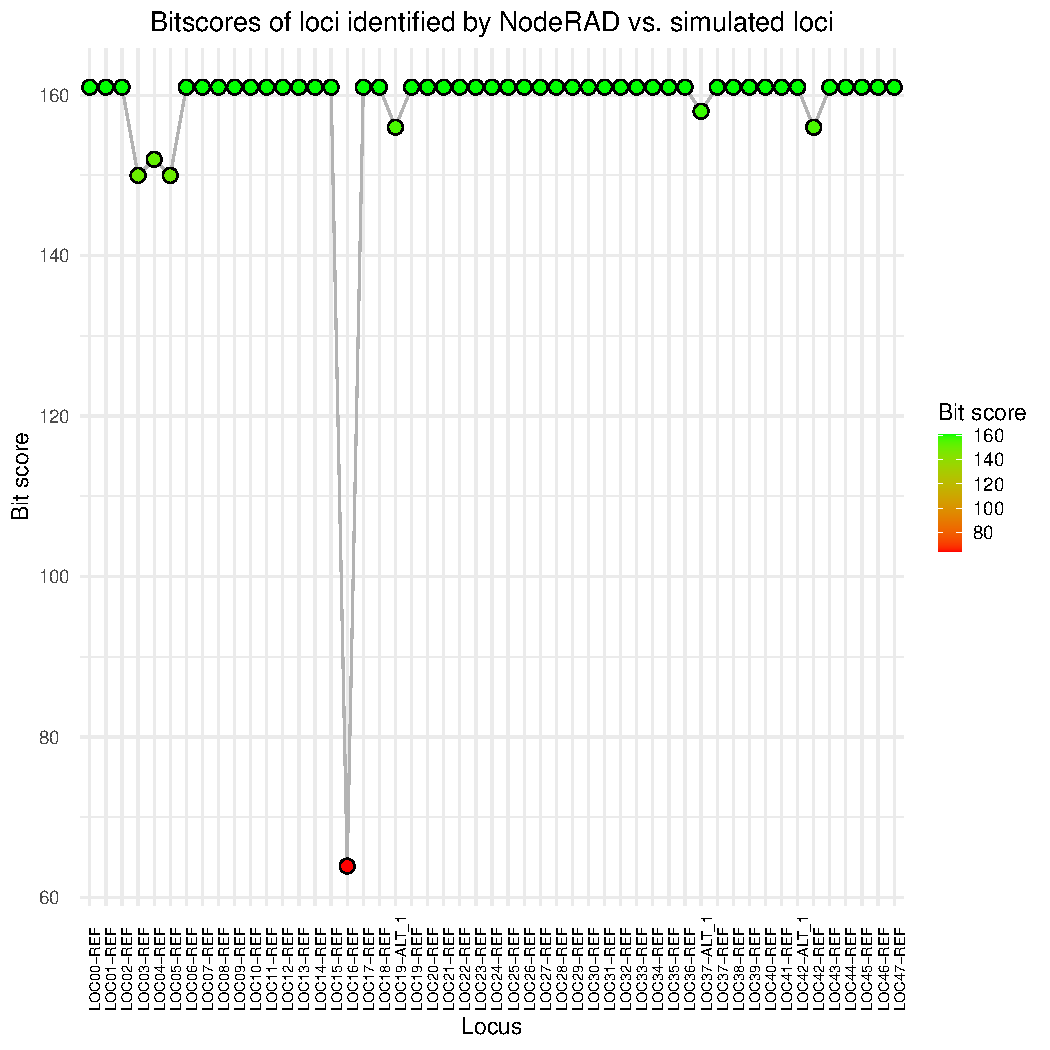
\includegraphics[height=16cm]{bilder/evaluation/bitscores/B.plot_bitscores.pdf}
		\caption{Individuum B: Bitscores aus dem Vergleich der durch NodeRAD bestimmten Loci mit den simulierten Loci}
	\end{center}
\end{figure}

\begin{figure}[H]
	\begin{center}
		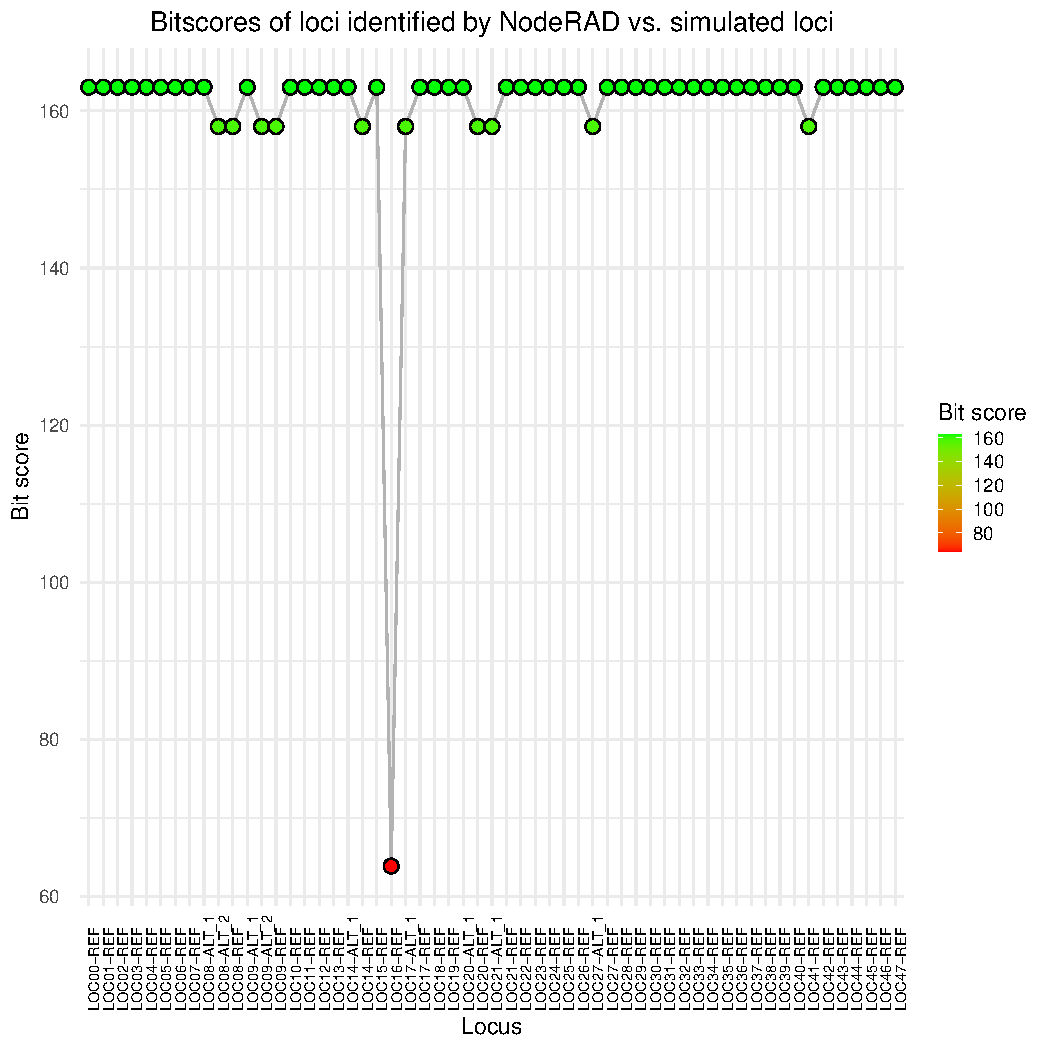
\includegraphics[height=16cm]{bilder/evaluation/bitscores/C.plot_bitscores.pdf}
		\caption{Individuum C: Bitscores aus dem Vergleich der durch NodeRAD bestimmten Loci mit den simulierten Loci}
	\end{center}
\end{figure}
